\section{Headroom Experiment}
\label{sec:headroom}
In this section, headroom experiment results are analyzed to guide our real hybrid prefetcher design. In section \ref{sec:headroomanalysis} we will talk about the potential of our design and the difference between two headroom test. In section \ref{sec:memorybandwidthissue}, one of the most influential factor, memory bandwidth, will be discussed in detail. Some other insights will be revealed in section \ref{sec:otherinsights}.

  \subsection{Headroom Result Analysis}
  \label{sec:headroomanalysis}

  \begin{figure}[ht!]
	   \centering
	   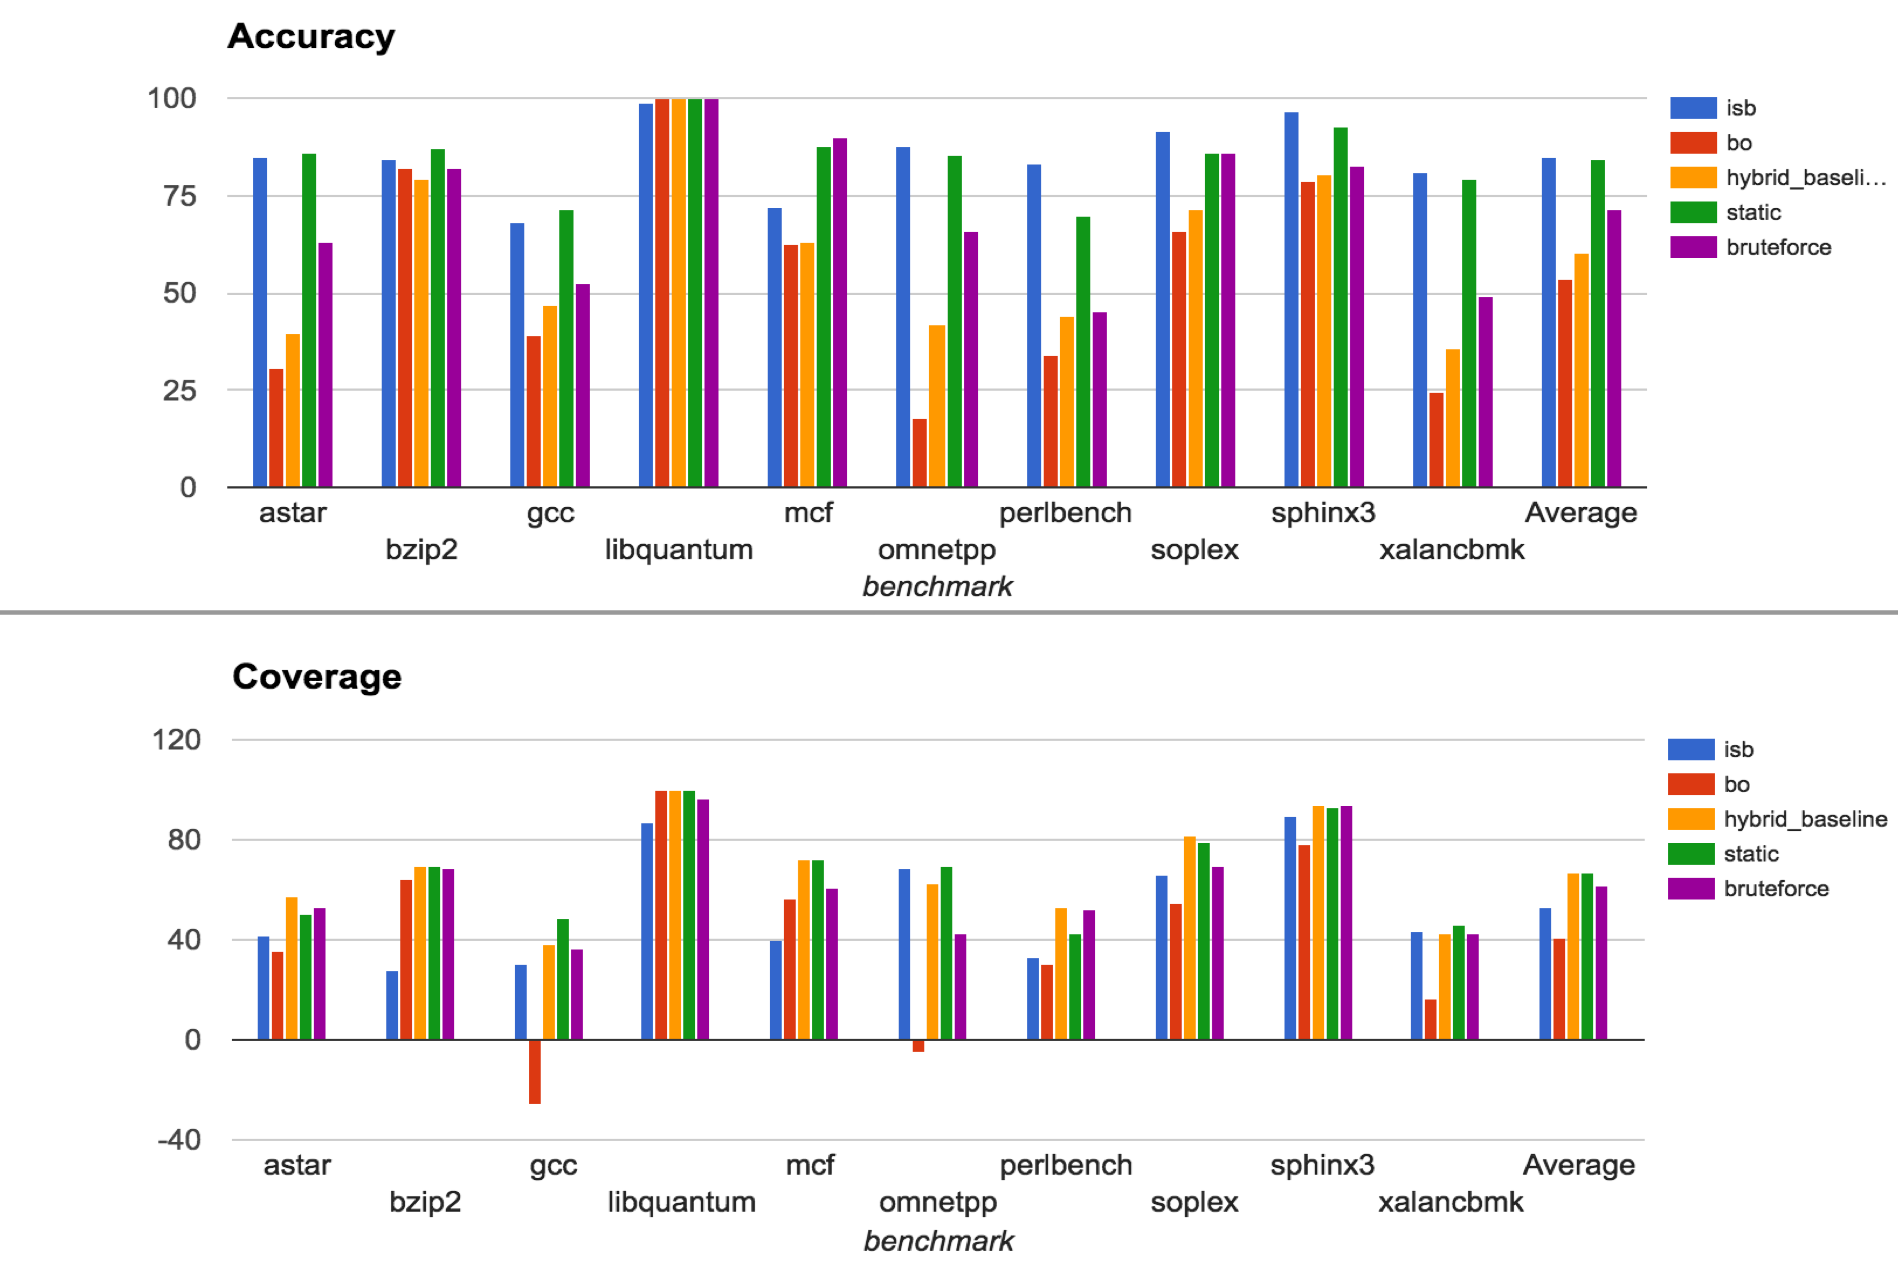
\includegraphics[width=1.0\textwidth]{images/headroom_acc_cov.png}
	   \caption{Headroom accuracy and coverage performance}
	  \label{fig:headroom_acc_cov}
  \end{figure}

  \begin{figure}[ht!]
	   \centering
	   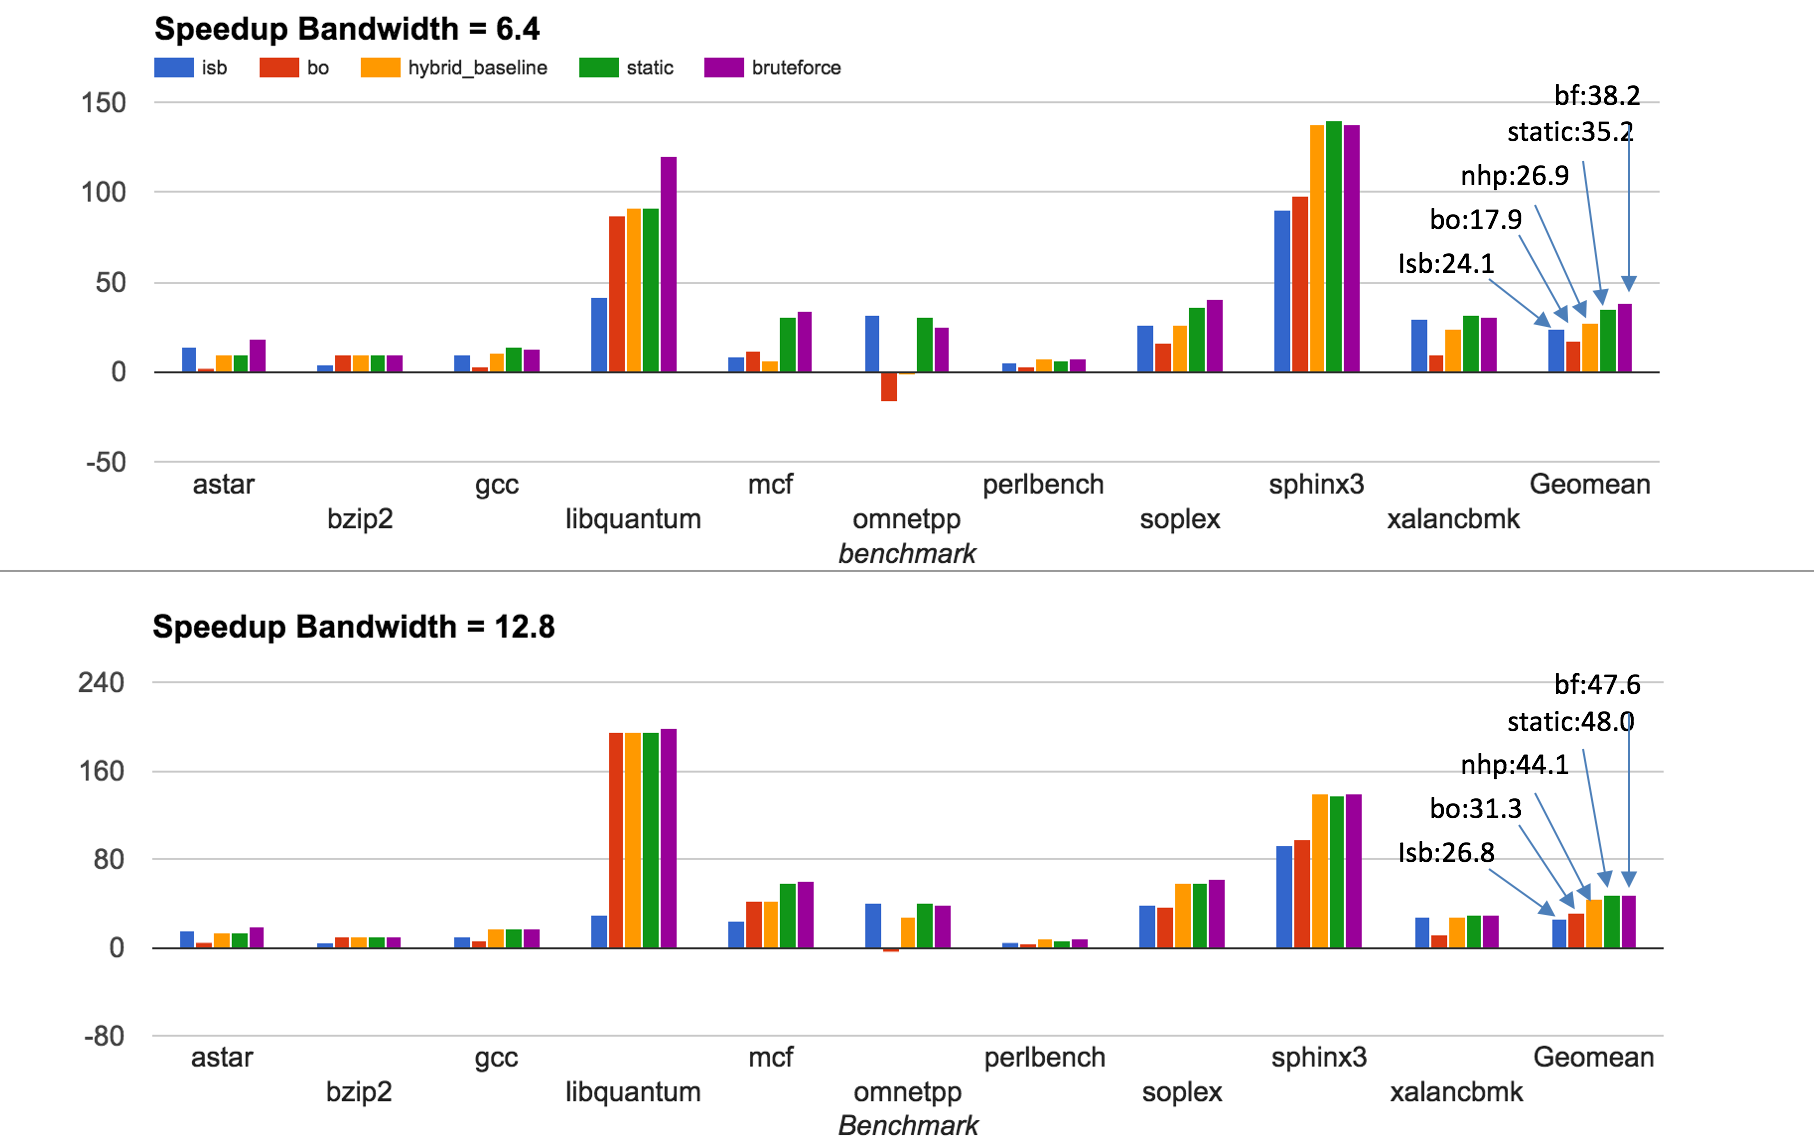
\includegraphics[width=1.0\textwidth]{images/headroom_speedup.png}
	   \caption{Headroom speedup under different memory bandwidth}
	  \label{fig:headroom_speedup}
  \end{figure}

  \subsection{Memory Bandwidth Issue}

  \label{sec:memorybandwidhissue}
  In Fig.\ref{fig:headroom_speedup}, the headroom of high bandwidth 12.8 GB/s is from NHB 44.1\% to static 48\%, it has about 3.9\% headroom. On low bandwidth 6.4 GB/s, the headroom is from NHB 26.9\% to BF 38.2\%, headroom is 11.3\%. 
  The figure shows that the headroom of hybrid prefetching system is highly related to memory bandwidth, and it is consistent with our previous discussion: hybrid prefetching system is limited by the amount of shared resources. 
  The less resources it has, the more headroom it can achieve.\par
  In this part we will discuss in detail how the memory bandwidth influences our performance, and how we can deal with it.\par

    \begin{figure}[ht!]
	   \centering
	   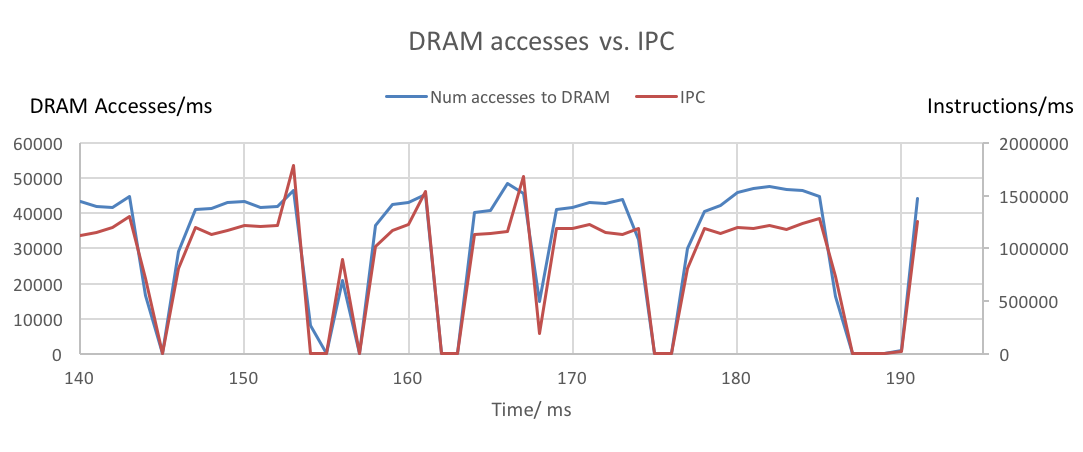
\includegraphics[width=1.0\textwidth]{images/bandwidth_IPC.png}
	   \caption{DRAM accesses vs IPC}
	  \label{fig:bandwidth_IPC}
  \end{figure}
  \begin{figure}[ht!]
	   \centering
	   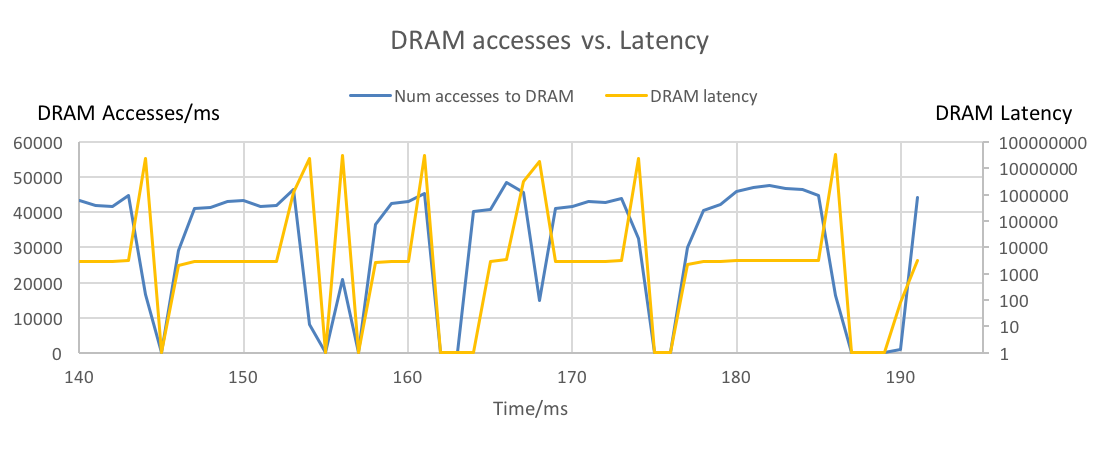
\includegraphics[width=1.0\textwidth]{images/bandwidth_latency.png}
	   \caption{DRAM accesses vs DRAM latency}
	  \label{fig:bandwidth_latency}
  \end{figure}

Fig.\ref{fig:bandwidth_IPC} and Fig.\ref{fig:bandwidth_latency} shows bandwidth, IPC and memory latency from benchmark \emph{astar} sim point 1 from 140ms to 192ms. The blue lines in both graphs are numbers of DRAM accesses per ms, which denotes the bandwidth usage. Red line is the number of executed instructions per ms, which denotes IPC. Yellow line is the sum of latency of all DRAM accesses per ms. X axis is the time line.\par
In Fig.\ref{fig:bandwidth_IPC}, DRAM accesses and IPC almost overlap. This indicates that at the low points, the benchmark program is stalled and DRAM doesn't receive any more request. For those low points in Fig.\ref{fig:bandwidth_latency}, latency increases a lot at the low points. Note that the latency Y axis is in log scale, the latency actually increases four to five magnitudes at those moments. The reason why the peak points of yellow is a little before the low points of blue is that, the sniper simulator calculates the latency of an access at the moment it is issued, not at the moment it returns.\par
 We can draw conclusions from these two figures that: 1) On some benchmarks, programs are occasionally stalled due to limited memory bandwidth and this is a significant issue to the performance. 2) Memory bandwidth should be considered in the hybrid prefetching system.  In our current headroom experiments, PCs make static decisions offline and never change decisions during execution. When we implement dynamic hybrid system, bandwidth usage is a factor to control the prefetching degree of prefetchers. \par


  \subsection{Some other insights}
  \label{sec:otherinsights}
